\section{\texorpdfstring{(Sub)gradient method on $\QG^+$-convex functions}{(Sub)-gradient method on QG+ convex functions}}
\label{apx:subgrad}

    In this appendix, we provide the proof of Theorems~\ref{thm:gd_average} and~\ref{thm:non_convergence_gd} stating respectively an upper bound result on the subgradient method with fixed step-size $1 / L$ on the Polyak-Rupert averaged iterate, and a lower bound result on the subgradient method on the last iterate.
    Finally, based on this lower bound, we suggest a specific tuning of the subgradient method for $\QG^+$ convex functions.
    A conjecture is formulated on the worst-case bound achieved by this method with the prescribed tuning, as well as evidence obtained through the PEP framework.
    
    \subsection{Convergence of subgradient method with fixed step-size at Polyak-Rupert averaged iterate}
    \label{apx:gd_proof_th1_upper_bound}

        In section~\ref{subsec:subgradient_method_on_qg+convex_functions}, we state the following theorem about a worst-case upper bound of \Cref{alg:subgrad} on the class of $\QG^+$-convex functions.
        In this section, we provide the proof of this theorem.
        
        \convergenceofsubgradientmethodinaverage*
    
        \noindent \textit{Proof.}
            Let $k \in [0, n]$.
            We have
            \begin{eqnarray*}
                d(x_{k+1}, \mathcal{X}_\star)^2 & = & \|x_{k+1} - \pi_{\mathcal{X}_\star}(x_{k+1})\|^2 \\
                & \leq & \|x_{k+1} - \pi_{\mathcal{X}_\star}(x_{k})\|^2 \\
                & = & \|x_k - \gamma g_k -  \pi_{\mathcal{X}_\star}(x_{k})\|^2, \qquad \text{ with } g_k \in \partial f(x_k) \\
                & = & \|x_k - \pi_{\mathcal{X}_\star}(x_{k})\|^2 - 2\gamma \left< x_k - \pi_{\mathcal{X}_\star}(x_{k}) , g_k \right> + \gamma^2 \|g_k\|^2 \\
                & \overset{Eq.~\eqref{eq:interp_convexity_qg}}{\leq} & \|x_k - \pi_{\mathcal{X}_\star}(x_{k})\|^2 - 2\gamma \left(f(x_k) - f_\star + \frac{1}{2L}\|g_k\|^2\right) + \gamma^2 \|g_k\|^2 \\
                & = & d(x_k, \mathcal{X}_\star)^2 - 2\gamma \left(f(x_k) - f_\star \right) - \gamma \left( \frac{1}{L} - \gamma \right) \|g_k\|^2 \\
                & \overset{\gamma=\frac{1}{L}}{=} & d(x_k, \mathcal{X}_\star)^2 - \frac{2}{L} \left(f(x_k) - f_\star \right)
            \end{eqnarray*}
            
            By reordering the terms and summing over $k$:
            \begin{equation}
                \sum_{k=0}^n (f(x_k) - f_\star) \leq \frac{L}{2}d(x_0, \mathcal{X}_\star)^2
            \end{equation}
            
            which leads to the desired results.
            
        $\hfill\blacksquare$
    
        \begin{Rem}
            \label{rem:gd_average}
            From Theorem~\ref{thm:gd_average}, we conclude
            \begin{eqnarray*}
                \min_{0 \leq k \leq n} f(x_k) - f_\star & \leq & \frac{L}{2}\frac{1}{n+1} d(x_0, \mathcal{X}_\star)^2 \\
                f\left( \frac{1}{n+1}\sum_{k=0}^n x_k \right) - f_\star & \overset{\text{(by convexity)}}{\leq} & \frac{L}{2}\frac{1}{n+1} d(x_0, \mathcal{X}_\star)^2.
            \end{eqnarray*}
        \end{Rem}
    
        \begin{Rem}
            Note that this bound is tight not only for $\QG^+$ convex functions, but also for smooth convex functions.
            
            Indeed, we consider the real Huber function defined as
            \begin{equation}
                \label{eq:huber}
                f(x) = \left\{
                \begin{array}{cc}
                    \frac{L}{2}x^2 & \text{if } |x| \leq 1 \\
                    L|x| - \frac{L}{2} & \text{if } |x| \geq 1
                \end{array}
                \right.
            \end{equation}
            
            This function is $L$-smooth convex and often used to find lower bounds~\citep[See e.g.][]{drori2014performance,taylor2017smooth,kim2016optimized}.
            Moreover, starting from $x_0 = n + 1$, GD with $\gamma = \frac{1}{L}$ leads exactly to $x_k = n+1-k$ for all $k\leq n$, hence $f(x_k) - f_\star = L \left(n+\frac{1}{2}-k\right)$ and $\sum_{k=0}^n (f(x_k) - f_\star) = L \sum_{k=0}^n n+\frac{1}{2}-k = \frac{L}{2}(n+1)^2 = \frac{L}{2}d(x_0, \mathcal{X}_\star)^2$.
        \end{Rem}
    
    \subsection{Convergence limitation of the subgradient method in last iterate}
    \label{apx:gd_lower_bound}

        In this section, we prove Theorem~\ref{thm:non_convergence_gd} stating a lower bound guarantee on the convergence of the subgradient method.
        This proof is by far the most technical of this paper due to the amount of newly introduced notations.
        
        \nonconvergenceofgdwithlowerboundedstepsizes*
        
        \noindent \textit{Proof.}
            Let $\eta > 0$.
            
            We introduce the following notations:
            \begin{itemize}
                \item $\delta \triangleq \left(\frac{\eta\sqrt{3}}{1+L\gamma_{n-2}}\right)^{1/2}$
                
                \item Huber function
                \begin{equation}
                    h_{\delta}(x) = 
                    \begin{cases}
                        \frac{L}{2}x^2 & \text{if } x \leq \delta \\
                        L \delta x - \frac{L}{2}\delta^2 & \text{if } x > \delta
                    \end{cases}
                    \label{eq:huber_functions}
                \end{equation}
        
                \item For $i \in [|0, n-1|]$, define $\xi_i \triangleq \delta \left( 1 + \sum_{k=i}^{n-2} L \gamma_i \right)$.
                
                \item $\lambda = \frac{L\eta}{(1 + L\gamma_{n-2})(1 + \eta^2 + \xi_0^2)}$.
            \end{itemize}
            
            Based on those notations, we define the $3$-dimensional function
            \begin{equation}
                f(x) = \max\left[\frac{L}{2}\left(x^{(1)} - 1 + |x^{(2)}|\sqrt{3}\right), h_{\delta}\left(x^{(3)}\right), \frac{\lambda}{2}\|x\|_2^2\right].
            \end{equation}
            
            $f$ is convex as maximum of 3 convex functions.
            
            Moreover, we note that $\mathcal{X}_\star = \lbrace 0 \rbrace$ and $f_\star = 0$.
            
            And each of the three components defining $f$ is smaller that $\frac{L}{2}\|x\|_2^2$.
            Indeed,
            \begin{align}
                \frac{L}{2}\left(x^{(1)} - 1 + |x^{(2)}|\sqrt{3}\right) & = \frac{L}{2}\left(\left(x^{(1)}\right)^2 - \left(x^{(1)} - \frac{1}{2}\right)^2 + \left(x^{(2)}\right)^2 - \left(x^{(2)} - \frac{\sqrt{3}}{2}\right)^2 \right) \nonumber \\
                & \leq \frac{L}{2} \left( \left(x^{(1)}\right)^2 + \left(x^{(2)}\right)^2 \right) \nonumber \\
                & \leq \frac{L}{2} \|x\|_2^2 \\
                h_{\delta}\left(x^{(3)}\right) & \leq \frac{L}{2}(x^{(3)})^2 \nonumber \\
                & \leq \frac{L}{2}\|x\|_2^2 \\
                \lambda & \leq \frac{L\eta}{2\eta} = \frac{L}{2} \leq L, \text{ hence }
                \frac{\lambda}{2}\|x\|_2^2 \leq \frac{L}{2}\|x\|_2^2
            \end{align}
            
            Therefore, $f$ is also $\QG^+(L)$.
            
            We choose to start the GD algorithm at $x_0 \triangleq \begin{pmatrix} 1 & \eta & \xi_0 \end{pmatrix}^\top$.
            
            We claim that after $i$ ($ 0 \leq i \leq n-1$) steps of GD, $x_i = \begin{pmatrix} 1 & \eta & \xi_i \end{pmatrix}^\top $.
            
            This can be proven by induction.
            Indeed, by definition, this is true for $i=0$.
            We now assume this property is true for some $i < n-1$ and want to prove it for $i+1$.
            
            From the 3 remarks
            \begin{align}
                h_{\delta}(\xi_i) & \geq \frac{L}{2}\left(1 - 1 + |\eta|\sqrt{3}\right) \\
                h_{\delta}(\xi_i) & \geq \frac{\lambda}{2}\|x_i\|_2^2 \\
                \xi_i & \geq \delta,
            \end{align}
            
            we conclude that $\nabla f(x_i) = \begin{pmatrix} 0 & 0 & L\delta \end{pmatrix}^\top$.
            
            Hence $x_{i+1} = x_i - \begin{pmatrix} 0 & 0 & L \gamma_i \delta \end{pmatrix}^\top = \begin{pmatrix} 1 & \eta & \xi_{i+1} \end{pmatrix}^\top$.
            
            Finally, from the 2 remarks
            \begin{align}
                \frac{L}{2}(1 - 1 + |\eta|\sqrt{3}) & \geq h_{\delta}(\xi_{n-1}) \\
                \frac{L}{2}(1 - 1 + |\eta|\sqrt{3}) & \geq \frac{\lambda}{2}\|x_{n-1}\|_2^2,
            \end{align}
            
            we conclude that $\nabla f(x_{n-1}) = \frac{L}{2} \begin{pmatrix} 1 & \sqrt{3} & 0 \end{pmatrix}^\top$, leading to $x_n = x_{n-1} - \gamma_{n-1} \frac{L}{2} \begin{pmatrix} 1 & \sqrt{3} & 0 \end{pmatrix}^\top = \begin{pmatrix} 1 - \frac{L\gamma_{n-1}}{2} & \eta - \frac{L\gamma_{n-1}\sqrt{3}}{2} & \delta \end{pmatrix}^\top$.
            
            We compute the two quantities
            \begin{align}
                \|x_0\|^2 & = 1 + \eta^2 + \xi_0^2 \\
                f(x_n) & \geq \frac{L}{2}\left(1 - \frac{L\gamma_{n-1}}{2} - 1 + |\eta - \frac{L\gamma_{n-1}\sqrt{3}}{2}|\sqrt{3}\right) \nonumber \\
                & = \frac{L}{2}\left(- \frac{L\gamma_{n-1}}{2} + \left(\frac{L\gamma_{n-1}\sqrt{3}}{2} - \eta\right)\sqrt{3}\right) \nonumber \\
                & = \frac{L}{2}\left(L\gamma_{n-1} - \eta\sqrt{3}\right)
            \end{align}
            
            Finally,
            
            \begin{align}
                \frac{f(x_n) - f_\star}{d(x_0, \mathcal{X}_\star)^2} & \geq \frac{L}{2} \frac{L\gamma_{n-1} - \eta\sqrt{3}}{1 + \eta^2 + \xi_0^2} \nonumber \\
                & = \frac{L}{2} \frac{L\gamma_{n-1} - \eta\sqrt{3}}{1 + \eta^2 + \delta^2 \left( 1 + \sum_{k=i}^{n-2} L \gamma_i \right)^2} \nonumber \\
                & = \frac{L}{2} \frac{L\gamma_{n-1} - \eta\sqrt{3}}{1 + \eta^2 + \frac{\eta\sqrt{3}}{1+L\gamma_{n-2}} \left( 1 + \sum_{k=i}^{n-2} L \gamma_i \right)^2} \nonumber \\
                & \underset{\eta \rightarrow 0}{\longrightarrow} \frac{L}{2}L\gamma_{n-1}.
            \end{align}
            
            Hence, for any $\epsilon >0$, we can find $\eta >0$ sufficiently small such that $f$ reaches the claim of the Theorem.
            
        $\hfill\blacksquare$

    \subsection{A new tuning prescription}
    \label{apx:gd_conjecture}

        Theorem~\ref{thm:non_convergence_gd} provides a lower bound on the last iterate value of the subgradient method on the class of $\QG^+$ convex functions.
        Moreover, a new analysis of the subgradient method on the Huber function~\eqref{eq:huber_functions}, starting at $x_0 = 1 + 2 \sum_{k=0}^{n-1} L\gamma_k$ provides another lower bound.
        
        Combining those 2 results, we know that whatever $(\gamma_i)_{0 \leq i \leq n-1}>0$ is, there exists $f$ an $L-\QG^+$ convex function as well as a starting point $x_0$ such that
        
        \begin{equation}
            \label{eq:gd_lower_bound}
            f(x_n) - f_\star \geq \max\left(\frac{L}{2}\frac{1}{1 + 2 \sum_{k=0}^{n-1} L\gamma_k}, \frac{L}{2}L\gamma_{n-1}\right) d(x_0, \mathcal{X}_\star)^2.
        \end{equation}

        Naturally, we propose the sequence of
        
        \begin{wrapfigure}[9]{R}{0.55\textwidth}
            \vspace{-1cm}
            \begin{minipage}{0.45\textwidth}
                \begin{algorithm}[H]
                    \caption{GD with decreasing step-sizes}\label{alg:gd_decreasing_step_sizes}
                    \KwInput{$x_0$, $L$}
                    $u_0 = 1$
                    
                    \For{k=1 \ldots n}{
                        $u_{k} \gets \frac{u_{k-1}}{2} + \sqrt{\left(\frac{u_{k-1}}{2}\right)^2 + 2}$;
                        
                        $\gamma_{k-1} \gets \frac{1}{L u_k}$;
                        
                        \text{Pick } $g_{k-1} \in \partial f(x_{k-1})$;
                        
                        $x_k \gets x_{k-1} - \gamma_{k-1} g_{k-1}$
                    }
                    \KwOutput{$x_n$}
                \end{algorithm}
            \end{minipage}
        \end{wrapfigure}

        \noindent $(\gamma_i)_{0 \leq i \leq n-1}>0$ that verifies for all $n$, $\frac{L}{2}\frac{1}{1 + 2 \sum_{k=0}^{n-1} L\gamma_k} = \frac{L}{2}L\gamma_{n-1}$ (for each index $n \geq 1$).
        This is summarized in Algorithm~\ref{alg:gd_decreasing_step_sizes}.
        We note that $u_n \sim 2\sqrt{n}$ and $\gamma_{n-1} \sim \frac{1}{2L\sqrt{n}}$.
        The lower bound~\eqref{eq:gd_lower_bound} for this method becomes $f(x_n) - f_\star \geq \frac{L}{2}L\gamma_{n-1} d(x_0, \mathcal{X}_\star)^2 \sim \frac{L}{4\sqrt{n}} d(x_0, \mathcal{X}_\star)^2$.
        We conjecture that this bound is actually reached by the proposed method~\ref{alg:gd_decreasing_step_sizes}.

        \begin{restatable}{Conj}{convergence_of_gd_with_decreasing_step-sizes}\textbf{\emph{(Convergence of GD with decreasing step-sizes)}}
            \label{conj:gd_sqrt}
            The algorithm~\ref{alg:gd_decreasing_step_sizes} verifies the following lower bound on every $L-\QG^+$ convex function $f$:
            \begin{equation}
                f(x_n) - f_\star \leq \frac{L}{2 u_n} d(x_0, \mathcal{X}_\star)^2.
            \end{equation}
            where $u_n$ is the sequence used in~\ref{alg:gd_decreasing_step_sizes}, defined by
            \begin{align}
                u_0 & = 1 \\
                u_{k} & = \frac{u_{k-1}}{2} + \sqrt{\left(\frac{u_{k-1}}{2}\right)^2 + 2}, \quad \text{for every } k \in \llbracket 1, n \rrbracket.
            \end{align}
            and verifying
            \begin{equation}
                u_n \sim 2\sqrt{n}.
            \end{equation}
        \end{restatable}

        This conjecture is supported by the Figure~\ref{fig:gd_sqrt} that has been built using the PEP framework.
        This figure represents the worst-case guarantee of Algorithm~\ref{alg:gd_decreasing_step_sizes} as a function of the number of iterations.
        The conjecture (red curve) follows exactly the numerical worst-case guarantee provided by the PEPs (blue curve) and the equivalent sequence (green curve) is very close to the 2 previous ones.
        
        \begin{figure}[h!]
            \centering
            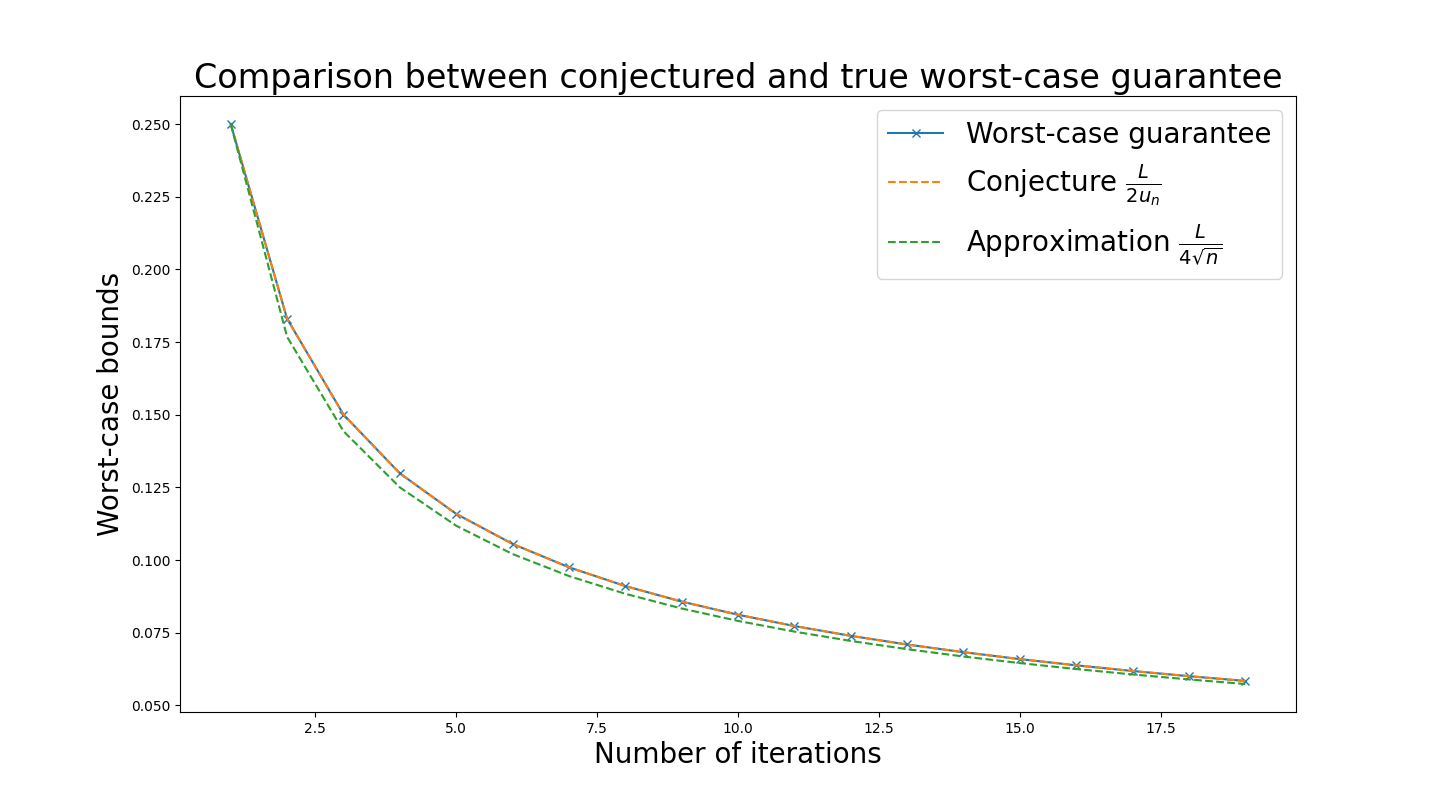
\includegraphics[width=0.9\textwidth]{Figure_1.png}
            \caption{Verification of the conjecture using PEPs}
            \label{fig:gd_sqrt}
        \end{figure}

\section{First-order lower bound}
\label{apx:lower_bound}

    In this section, we prove the lower bound of first order methods on $\QG^+$ convex functions.
    
    In the first subsection, we assume that the iterates of the first order algorithm must stay in the span of the past observed gradients.
    
    In the second subsection, we release this assumption and still prove the same lower bound.
    This proof is a bit more technical, hence the reason why we provide the two proofs.
    
    \subsection{\texorpdfstring{Proof of Theorem 2.3}{Proof of Theorem~\ref{thm:general_lower_bound}}}
    \label{apx:lower_bound_1}

        The following theorem brings a lower bound over all first order methods verifying that all the iterates lie into the span of the previously observed gradients.
        
        \lowerboundoffirstorderalgorithm*
        
        \noindent \textit{Proof.}
            Consider $f(x) \triangleq \frac{L}{2}\|x\|_\infty^2$ defined on $\mathbb{R}^{n+1}$ and $x_0=\Vec{\mathbf{1}}$.
            
            After $k$ steps, the oracle can ``choose'' to return a vector that lies in the first $k+1$ dimension of the input space, leading to $f(x_n) - f_\star \geq f(x_0) - f_\star = \frac{L}{2} = \frac{L}{2}\frac{1}{n+1} d(x_0, \mathcal{X}_\star)^2$.
        $\hfill\blacksquare$

        \begin{Rem}
            Note that by considering instead $x_0 = \begin{pmatrix}
                1 & 1 - \varepsilon/n & 1 - 2\varepsilon/n & \ldots & 1 - \varepsilon
            \end{pmatrix}^\top$,
            one ends up with $f(x_n) - f_\star \geq \frac{L}{2}\frac{1 - \varepsilon}{n+1} d(x_0, \mathcal{X}_\star)^2$ \textbf{whatever} the oracle ``chooses'' to return.
        \end{Rem}

    \subsection{Lower bound proof without span assumption}
    \label{apx:lower_bound_2}

        In this section we release the span assumption and prove that the previously shown lower bound still holds.
        This proof is a bit more technical than the one of Theorem~\ref{thm:general_lower_bound} proven in Appendix~\ref{apx:lower_bound_1}.
        
        \begin{Th}[Lower bound of first order algorithm without span assumption]
            Let $\mathcal{A}$ a first-order algorithm.
            Then, for any $n \geq 0$, there exists $d$ a positive integer, $f$ a $L-\QG^+$ convex function of input space $\mathbb{R}^d$ and a starting point $x_0$ such that $f(x_n) - f_\star \geq \frac{L}{2}\frac{1}{n+1} d(x_0, \mathcal{X}_\star)^2$.
        \end{Th}
        
        \noindent \textit{Proof.}
            Let $\mathcal{E} = \left\{ v \in \mathbb{R}^{n+1} | \forall i \in \llbracket 1, n+1 \rrbracket, |v_i| = 1 \right\}$ the set of the $2^{n+1}$ vectors of $\mathbb{R}^{n+1}$ which all coordinates are $\pm 1$.
            
            For each $v\in\mathcal{E}$, we introduce $f_v(x) \triangleq \frac{L}{2}\|x - v\|_\infty^2$ defined on $\mathbb{R}^{n+1}$.
            
            First note that all those functions are $L-\QG^+$ convex.
            We will prove that not only there exists a starting point $x_0$ and a $L-\QG^+$ convex function such that $f(x_n) - f_\star \geq \frac{L}{2}\frac{1}{n+1} d(x_0, \mathcal{X}_\star)^2$, but also that there exists a starting point $x_0$ and a function among the $f_v$ we introduced above such that the latest holds.
            
            To proceed, we need to show that the algorithm $\mathcal{A}$ cannot know the right $v$ after only $n$ iterations and therefore, cannot guarantee $f(x_n) - f_\star \leq \frac{L}{2}$.
            Taking $x_0 = \Vec{0}$, $\|x_0 - x_\star \|^2 = n+1$ whatever $x_\star$ is (among $\mathcal{E}$), hence the result.
            
            In order to prove that the algorithm cannot know the solution after $n$ iterations, we keep track of all the remaining possibilities across time.
            
            We denote by $\mathcal{E}_k$ the remaining possibilities after $k$ steps of the algorithm.
            In particular, $\mathcal{E}_0=\mathcal{E}$.
            
            At each step $k$, $\mathcal{A}$ guesses $x_k$ based on all the previous information, summarized in $\mathcal{E}_k$, and the oracle provides $f(x_k)$ and a sub-gradient $g_k \in \partial f(x_k)$.
            
            Let $v_k \in \arg\max_{v \in \mathcal{E}_k} \|x_k - v_k\|_\infty$.
            We consider the case where the oracle behaves like if the objective function to minimize was $f_{v_k}$.
            Moreover, in the case where $f_{v_k}$ is not differentiable in $x_k$, we ask that the oracle returns a sub-gradient co-linear to a vector belonging to the canonical basis (which is always possible).
            
            Considering $i$ such that $g_k$ is co-linear to $e_i$, we obtain
            $\mathcal{E}_{k+1} = \left\{ v \in \mathcal{E}_k | \left< v, e_i \right> = \left< v_k, e_i \right> \right\}$, reducing by half the number of remaining elements at each step (except when the algorithm badly guesses and receive twice the same direction, in which case one of the steps is useless).
            
            After $n$ steps, $\mathcal{E}_{n}$ contains 2 elements, and the algorithm $\mathcal{A}$ must guess based on nothing.
            Again, we consider the further one to the last guess as the right solution, and obtain the lower bound provided by the Theorem.
            
        $\hfill\blacksquare$

\section{Main result: worst-case guarantee of proposed methods}
\label{apx:main_result}

    In this section, we prove Theorem~\ref{thm:main}, the main result of this paper, stating that all the sequences of iterates verifying a certain property enjoy an upper bound guarantee corresponding to the lower bound presented in \Cref{thm:general_lower_bound} and proved in \Cref{apx:lower_bound}.
    
    \mainresult*
    
    \noindent \textit{Proof.}
        This proof relies on the Lyapunov function
        \begin{equation}
            V_n \triangleq n(f(x_{n-1}) - f_\star) + \frac{L}{2} \left\| x_0 - \pi_{\mathcal{X_\star}}(x_0) - \sum_{i=0}^{n-1}\frac{1}{L}g_i \right\|^2.
        \end{equation}
        
        For all $k$, we verify
        
        \begin{eqnarray*}
            V_{k+1} - V_k & = & \left[(k+1)(f(x_{k}) - f_\star) + \frac{L}{2} \left\| x_0 - \pi_{\mathcal{X_\star}}(x_0) - \sum_{i=0}^{k}\frac{1}{L}g_i \right\|^2 \right] \\
            & & - \left[k(f(x_{k-1}) - f_\star) + \frac{L}{2} \left\| x_0 - \pi_{\mathcal{X_\star}}(x_0) - \sum_{i=0}^{k-1}\frac{1}{L} g_i \right\|^2 \right] \\
            & = & (f(x_k) - f_\star) + k(f(x_k) - f(x_{k-1})) + \frac{L}{2} \left[ -\frac{2}{L} \left< g_k , x_0 - \pi_{\mathcal{X_\star}}(x_0) - \sum_{i=0}^{k-1}\frac{1}{L} g_i \right> + \frac{1}{L^2} \|g_k\|^2 \right] \\
            & = & \left(f(x_k) - f_\star + \frac{1}{2L} \|g_k\|^2\right) + k(f(x_k) - f(x_{k-1})) - \left< g_k , x_0 - \pi_{\mathcal{X_\star}}(x_0) - \sum_{i=0}^{k-1}\frac{1}{L} g_i \right> \\
            & \overset{(\ref{eq:interp_convexity},~\ref{eq:interp_convexity_qg})}{\leq} & \left< g_k , x_k - \pi_{\mathcal{X_\star}}(x_0) \right> + k\left< g_k , x_k - x_{k-1} \right> - \left< g_k , x_0 - \pi_{\mathcal{X_\star}}(x_0) - \sum_{i=0}^{k-1}\frac{1}{L} g_i \right> \\
            & = & \left< g_k , x_k - \pi_{\mathcal{X_\star}}(x_0) + k(x_k - x_{k-1}) - \left( x_0 - \pi_{\mathcal{X_\star}}(x_0) - \sum_{i=0}^{k-1}\frac{1}{L} g_i \right) \right> \\
            & = & \left< g_k , (k+1) x_k - k x_{k-1} - x_0 + \sum_{i=0}^{k-1}\frac{1}{L} g_i \right>
        \end{eqnarray*}
        
        The assumption therefore concludes
        \begin{equation*}
            \forall k, V_{k+1} \leq V_k
        \end{equation*}
        
        Finally,
        
        \begin{equation*}
            (N+1)(f(x_{N}) - f_\star) + \frac{L}{2} \left\| x_0 - \pi_{\mathcal{X_\star}}(x_0) - \sum_{i=0}^{N}\frac{1}{L} g_i \right\|^2 = V_{n+1} \leq V_0 = \frac{L}{2}\|x_0 - x^*\|^2.
        \end{equation*}
        
        Hence,
        
        \begin{equation*}
            f(x_{N}) - f_\star \leq \frac{L}{2}\frac{1}{N+1}\|x_0 - x^*\|^2.
        \end{equation*}
        
    $\hfill\blacksquare$

\section{\texorpdfstring{Summary of convergence results on $\QG^+$ convex and Lipschitz convex}{Summary of convergence results on QG+ convex and Lipschitz convex}}
\label{apx:tab}

    In this section, we state and prove the 2 results of \Cref{tab:optimality_summary} that are not already proven elsewhere.
    
    \addtocounter{table}{-1}
    
    \begin{table*}
        {
        \caption{
            Optimality of the proposed methods over the set of $\QG^+$ convex functions and $M$-Lipschitz convex functions.
            ELS: Exact Line-Search. $\cmark$ indicates optimality among the class and $\xmark$ the contrary.
            All counter examples are given in App.~\ref{apx:tab}. $\ ^{\dagger}$:~constants resulting in optimal convergence rates depend on the class, thus for example heavy-ball with step-size $\frac{\text{constant}}{(t+2)}$ is not adaptive as it does not achieve the optimal rate for both classes with the same constant. $\ ^\ddagger$: up to a $\log$ factor.
            } \vspace{-0.3cm}
        \begin{center}
            {\renewcommand{\arraystretch}{1.8}
            \resizebox{\linewidth}{!}{
             \begin{tabular}{@{}lllcrcrc@{}}
                \specialrule{2pt}{1pt}{1pt}
                \multicolumn{3}{c}{Method} & \multicolumn{4}{c}{Function class} & Parameter free \\
                 \cmidrule{1-3}\cmidrule(l){4-7}\cmidrule(l){8-8}
                Algorithm & Step-sizes $(\gamma_t)_{0\le t\le n-1}$  & Iterate & \multicolumn{2}{c}{$\QG^+(L)$ convex} & \multicolumn{2}{c}{$M$-Lipschitz convex}   \\
                \cmidrule(l){4-5}\cmidrule(l){6-7}
                Subgradient (Alg.~\ref{alg:subgrad}) & $\text{constant}^{\dagger}$ & Average &  $\cmark$ & (Thm.~\ref{thm:gd_average}) & $ \xmark$ & (Thm.~\ref{thm:subgrad_constant_lower_lip}) & $\xmark$ \\
                Subgradient (Alg.~\ref{alg:gd_decreasing_step_sizes}) & $ \text{constant}^{\dagger}/\sqrt{t}$ & Average & $\xmark$ &~\eqref{eq:LB_smooth} & $\cmark^\ddagger$ &~\citep[Sec. 3.2.3]{Nest03a} & $\xmark$ \\
                Subgradient (Alg.~\ref{alg:subgrad_els}) & ELS & Average &  $\xmark$ & (Thm.~\ref{thm:gd_els_lower_bound}) & $\xmark$ & (Thm.~\ref{thm:gd_els_lower_bound}) & $\cmark$ \\
                Subgradient (Alg.~\ref{alg:subgrad_els}) & ELS & Last &  $\xmark$ & (Thm.~\ref{thm:gd_els_lower_bound}) & $\xmark$ & (Thm.~\ref{thm:gd_els_lower_bound}) & $\cmark$ \\
                \midrule
                Heavy-ball (Alg.~\ref{alg:ogm}) & $\text{constant}^{\dagger}/(t+2)$ & Last & $\cmark$ & (Cor.~\ref{cor:optimal}) & $\cmark$ &~\citep[][, Cor. 3]{drori2020efficient} & $\xmark$ \\
                Heavy-ball (Alg.~\ref{alg:ogm_ls}) & ELS & Last & $\cmark$ & (Cor.~\ref{cor:optimal}) & $\cmark$ &~\citep[][, Cor. 4]{drori2020efficient} & $\cmark$ \\
                \specialrule{2pt}{1pt}{1pt}\vspace{0em}
            \end{tabular}}
            \vspace{-1cm}
            }
        \end{center}}
    \end{table*}
    
    We first state \Cref{thm:subgrad_constant_lower_lip}.
    
    \begin{Th}
        For any $M>0$ and any $\gamma>0$, the subgradient method~\ref{alg:subgrad} with constant step-size $\gamma$ cannot be guaranteed to converge to optimum on all the $M$-Lipschitz continuous convex functions, both in last iterate and in Polyak-Rupert averaged iterate.
        \label{thm:subgrad_constant_lower_lip}
    \end{Th}

    \noindent \textit{Proof.}
        First we note that $f \triangleq z \mapsto M |z|$ is $M$-Lipschitz continuous and convex.
        Let $\gamma>0$.
        We consider $x_0 = \frac{3}{4}M\gamma$ the starting point of the subgradient method with constant step-size $\gamma$.
        We verify that $x_1 = -\frac{1}{4}M\gamma$ and that the sequence $(x_t)_t$ cycles back to $\frac{3}{4}M\gamma$.
        Therefore, the sequence itself does not converge and the sequence of the PR averaged iterates converges to $\frac{1}{4}M\gamma$, while the optimum value would be 0.
    $\hfill\blacksquare$

    \begin{wrapfigure}[6]{R}{0.56\textwidth}
        \begin{minipage}{0.56\textwidth}
            \vspace{-1.0cm}
            \begin{algorithm}[H]
                \caption{Subgradient method with line-search \label{alg:subgrad_els}}
                \KwInput{$x_0$, $v_0 \gets 0$}
                \For{$k=1 \ldots n$}{
                    \text{Pick } $g_{k-1} \in \partial f(x_{k-1})$.
                    
                    $\alpha_k \gets \arg\min_{\alpha} f\left( x_{k-1} - \alpha g_{k-1} \right)$
                    
                    $x_k \gets x_{k-1} - \alpha_k g_{k-1}$
                }
                \KwOutput{$x_n$}
            \end{algorithm}
        \end{minipage}
    \end{wrapfigure}

    Then, one could wonder whether performing exact line search steps on the subgradient method (Algorithm~\ref{alg:subgrad_els}.) leads to convergence on Lipschitz continuous convex or $\QG^+$ convex function.
    We now prove Theorem~\ref{thm:gd_els_lower_bound} stating that the subgradient method with exact line search does not converge for all functions neither of the class of Lipschitz continuous convex functions nor of the class of $\QG^+$ convex functions, neither in last iterate nor in Polyak-Rupert averaged iterate.
    
    \begin{Th}
        There exists a $\QG^+$ convex function $f_{QG}$ and a Lipschitz continuous convex function $f_{Lip}$ such that, the iterates $((x_n)_n^{f_{QG}})_n$ and $((x_n)_n^{f_{Lip}})_n$ obtained by Algorithm~\ref{alg:subgrad_els}, verify the 2 guarantees
        
        \begin{align}
            f(x_n) - f_\star & \geq && \frac{L}{6} \|x_0 - x_\star\|^2. \\
            f(\bar{x_n}) - f_\star & \geq && \frac{L}{6} \|x_0 - x_\star\|^2.
        \end{align}
        
        where $\bar{x_n}$ denotes the Polyak-Rupert averaged iterate obtained from the sequence $(x_n)_n$.
        
        \label{thm:gd_els_lower_bound}
    \end{Th}

    \noindent \textit{Proof.}
        Considering $f_{Lip}(z) = M\|x\|_\infty$ and $f_{QG}(z) = \frac{L}{2}\|x\|_\infty^2$ defined on $\mathbb{R}^3$,
        the iterates of Algorithm~\ref{alg:subgrad_els} can be cycling between the four points $(1,1,1)$, $(1,-1,1)$, $(-1,1,1)$ and $(-1,-1,1)$.
        Therefore, the aforementioned statement.
    $\hfill\blacksquare$
    
\vspace{.5cm}

\section{\texorpdfstring{Interpolation results for $\QG^+$ convex functions}{Interpolation results for QG+ convex functions}}
\label{apx:interpolation_conditions}

    The interpolation conditions of a given class represent the key ingredient to use the PEP framework on this class.
    Theorem~\ref{thm:interp} provides the interpolation conditions for the class of $\QG^+$ convex functions.
    In this section, we recall this result and prove it.

    \interpolationconditions*

    \noindent \textit{Proof.}

        We prove the two implications one by one.

        \begin{itemize}
            \item[$\Rightarrow$:] Assume there exists such a convex-$\QG^+$ function $f$ that interpolates $(x_i, g_i, f_i)_{i \in I}$.
            Equation~\eqref{eq:interp_convexity} follows immediately from convexity.
            Let's prove equation~\eqref{eq:interp_convexity_qg}.
            Let $i \in I_\star, \forall j \in I$ and $x \in \mathbb{R}^d$.
            We have:
            \begin{equation*}
                f_j + \left< g_j, x - x_j \right> \overset{\text{CVX}}{\leq} f(x) \overset{\QG^+}{\leq} \min_{z \in \mathbb{R}^d} f(z) + \frac{L}{2}d(x, \mathcal{X}_\star)^2 \leq f_i + \frac{L}{2}\|x - x_i \|^2.
            \end{equation*}
            Rewriting the previous equation for $x = x_i + \frac{1}{L}g_j$ leads to equation~\eqref{eq:interp_convexity_qg}.

            \item[$\Leftarrow$:] Let's consider equations~\eqref{eq:interp_convexity} and~\eqref{eq:interp_convexity_qg} are verified.
            Applying~\eqref{eq:interp_convexity} with $j \in I_\star$
            \begin{equation}
                \forall i \in I, \forall j \in I_\star, f_i \geq f_j \label{eq:stationary_are_minima}
            \end{equation}
            In particular, $\forall i \in I_\star, \forall j \in I_\star, f_i = f_j$.
            Hence, let's introduce $f_\star$ the common value of all the $f_i$ for $i \in I_\star$.
            Let's denote here $\mathcal{X}^\star$ the convex hull of $\left\{x_i\right\}_{i \in I_\star}$.
            Finally let's introduce $\mu \triangleq 2 \min_{i \in I \setminus I_\star} \left( \frac{f_i - f_\star}{d(x_i, \mathcal{X}^\star)^2} \right)$.

            Let's prove that the following function $f$ is a solution:
            \begin{equation}
                f(x) = \max\left( \max_{j \in I} \left( f_j + \left< g_j, x - x_j \right> \right), f_\star + \frac{\mu}{2}d\left(x, \mathcal{X}^\star \right)^2 \right).
                \label{eq:interpolation_function}
            \end{equation}

            \begin{itemize}
                \item[-]\underline{$\forall i \in I, f(x_i) = f_i$:} For all $i \in I$, equation~\eqref{eq:interp_convexity} shows $\max_{j \in I} \left( f_j + \left< g_j, x_i - x_j \right> \right) \leq f_i$ and the definition of $\mu$ leads to $f_\star + \frac{\mu}{2}d\left(x_i, \mathcal{X}^\star \right)^2 \leq f_i$.
                Hence, for all $i \in I$, $f(x_i) \leq f_i$.
                Moreover, from equation~\eqref{eq:interpolation_function}, $f(x) \geq \left( f_i + \left< g_i, x - x_i \right> \right)$, hence $f(x_i) \geq f_i$.
                Finally, we conclude $\forall i \in I, f(x_i) = f_i$.

                \item[-]\underline{$\forall i \in I, g_i \in \partial f(x_i)$:} $\forall i \in I, f(x) \geq \left( f_i + \left< g_i, x - x_i \right> \right)$, and from the previous point, we conclude $\forall i \in I, f(x) \geq \left( f(x_i) + \left< g_i, x - x_i \right> \right)$.
                Finally, $\forall i \in I, g_i \in \partial f(x_i)$.

                \item[-]\underline{$f$ is convex:} $f$ is clearly defined as the maximum of convex functions, hence is convex.

                \item[-]\underline{$f$ is $\QG^+$:} We aim at proving that $\forall x \in \mathbb{R}^d, f(x) \leq f_\star + \frac{L}{2}d\left(x, \mathcal{X}^\star \right)^2$.
                Since it is clear that $\forall x \in \mathbb{R}^d, f_\star + \frac{\mu}{2}d\left(x, \mathcal{X}^\star \right)^2 \leq f_\star + \frac{L}{2}d\left(x, \mathcal{X}^\star \right)^2$, it remains to prove that
                $\forall x \in \mathbb{R}^d, \forall j \in I, f_j + \left< g_j, x - x_j \right> \leq f_\star + \frac{L}{2}d\left(x, \mathcal{X}^\star \right)^2 $.
                The latest is also equivalent to $\forall x \in \mathbb{R}^d, \forall j \in I, \forall x_\star \in \mathcal{X}^\star, f_j + \left< g_j, x - x_j \right> \leq f_\star + \frac{L}{2}\| x - x_\star \|^2 $.
                For $j$ and $x_\star$ fixed, this expression is a quadratic form in $x$, optimized for $x = x_\star + \frac{1}{L}g_j$.
                Hence, we need to show $\forall j \in I, \forall x_\star \in \mathcal{X}^\star, f_j + \left< g_j, x_\star + \frac{1}{L}g_j - x_j \right> \leq f_\star + \frac{L}{2}\left\| x_\star + \frac{1}{L}g_j - x_\star \right\|^2 $, also rewritten $\forall x_\star \in \mathcal{X}^\star, \forall j \in I, f_\star \geq f_j + \left< g_j, x_\star - x_j \right> + \frac{1}{2L} \|g_j\|^2$.
                Since $\mathcal{X}^\star$ is the convex hull of $\left\{ x_i \right\}_{i \in I_\star}$, the latest is obtained by linear combination (with non-negative weights) of equation~\ref{eq:interp_convexity_qg} for different values of $i$.
            \end{itemize}
        \end{itemize}
    $\hfill\blacksquare$


\section{Convergence bound on other classes}
\label{apx:upper_assumption}

    In this section, we naturally extend the previous results to the class of $h-\RG^+$ (See. \Cref{def:h_rg}) convex functions.

    \hbgeneral*

    \noindent \textit{Proof.}

        First note that since $h$ is strictly increasing, $h^{-1}$ is well defined.
        Furthermore, Definition~\ref{def:h_rg} can be expressed as
        $h^{-1}\left(f(x)-f_\star\right) \leq d(x, \mathcal{X}_\star)^2.$
        Therefore, $h^{-1}\left(f-f_\star\right)$ is $2-\QG^+$.
        And we know by definition that $h$ is increasing and concave, then $h^{-1}$ is increasing and convex.
        Since $f$ is also convex, so is $h^{-1}\left(f-f_\star\right)$.

        We conclude that $h^{-1}\left(f-f_\star\right)$ is $2-\QG^+$ and convex, and then we know that Algorithm~\ref{alg:hb_ogm} applied on $h^{-1}\left(f-f_\star\right)$ leads to

        \begin{equation*}
            h^{-1}\left(f(x_n) - f_\star\right) \leq \frac{d(x_0, \mathcal{X}_\star)^2}{n+1}.
        \end{equation*}

        It remains to compose the above by $h$ and to notice that Algorithm~\ref{alg:hb_ogm} applied on $h^{-1}\left(f-f_\star\right)$ is exactly Algorithm~\ref{alg:hb_general}.

    $\hfill\blacksquare$

\section{Linear convergence guarantees under lower bound assumption}
\label{apx:restart}

    In all this section, we assume that $f$ is convex and $h-\RG^+$ for a certain $h$.
    Moreover, we consider that $f$ verifies the following additional assumption (referred to as ``\L{}ojasiewicz error bound inequality'' in~\citep{bolte2017error}) for a given $\kappa \geq 1$:

    \begin{Assump}
        \label{assump:h_kappa}
        For all $x \in \mathbb{R}^d$, $f(x)-f_\star \geq h\left( \frac{ d(x, \mathcal{X}_\star)^2}{\kappa} \right)$.
    \end{Assump}

    \begin{Rem}
        When $h$ is the linear function $h: R \mapsto \frac{LR}{2}$, then $f$ is simply $L-\QG^+$ convex as well as $\mu-\QG^-$ $\left(\text{where } \mu \triangleq \frac{L}{\kappa}\right)$(See~\citep{guille2021study} for the definition of $\QG^-$).
    \end{Rem}

    We introduce the following algorithm based on the restart idea studied in~\citep{nemirovskii1985optimal, nesterov2013gradient, iouditski2014primal}.

    \begin{algorithm}
        \caption{Heavy-ball with restart}
        \label{alg:hb_restart}
        \KwInput{$x_0$, $h$, $f_\star$}
        \For{$k=1 \ldots n$}{
        Choose ~ $g_{k-1}$ from $\partial f(x_{k-1})$

        $l \gets k \text{ mod } \left\lfloor \kappa e \right\rfloor - 1 $ \quad (between $1$ and $\left\lfloor \kappa e \right\rfloor - 1$).

        $x_k \gets x_{k-1} - \frac{1}{2(l+1)}\frac{1}{h' \circ h^{-1}\left(f(x_{k-1}) - f_\star\right)} g_{k-1} + \frac{l-1}{l+1}\left( x_{k-1} - x_{k-2} \right) $
        }
        \KwOutput{$x_n$}
    \end{algorithm}

    This algorithm comes with the linear convergence rate guarantee

    \begin{center}
        \fbox{\parbox{\textwidth}{
        \begin{restatable}{Th}{hbrestart}\textbf{\emph{}}
            \label{thm:hb_restart}
            Algorithm~\ref{alg:hb_restart} verifies for every $n$ multiple of $\left\lfloor \kappa e \right\rfloor - 1$:

            \begin{equation}
                d(x_n, \mathcal{X}_\star)^2 \leq \left(1 - \frac{1}{\kappa e}\right)^n d(x_0, \mathcal{X}_\star)^2.
            \end{equation}
        \end{restatable}
        }}
    \end{center}

    \noindent \textit{Proof.}

        From Theorem~\ref{thm:hb_general}, running Algorithm~\ref{alg:hb_general} leads to the guarantee
        \begin{equation}
            f(x_n) - f_\star \leq h\left(\frac{d\left(x_0, \mathcal{X}_\star\right)^2}{n+1} \right).
        \end{equation}

        From the additional assumption (\ref{assump:h_kappa}), we can upper bound the left hand size of the above and write
        \begin{equation*}
            h\left( \frac{ d(x_n, \mathcal{X}_\star)^2}{\kappa} \right) \leq h\left(\frac{d\left(x_0, \mathcal{X}_\star\right)^2}{n+1} \right).
        \end{equation*}

        Hence,
        \begin{equation*}
            d(x_n, \mathcal{X}_\star)^2 \leq \frac{\kappa}{n+1}d(x_0, \mathcal{X}_\star)^2.
        \end{equation*}

        The latest is a contraction guarantee.
        Indeed, for $n$ sufficiently large, $d(x_n, \mathcal{X}_\star)^2 < d(x_0, \mathcal{X}_\star)^2$.
        The average contraction factor is $\left(\frac{\kappa}{n+1}\right)^{1/n}$ and is minimized for $n \approx \left\lfloor \kappa e \right\rfloor - 1$.
        Choosing such a $n$ leads to a contraction factor upper bounded by $1 - \frac{1}{\kappa e}$.

        This corresponds to the convergence rate obtained by applying $\left\lfloor \kappa e \right\rfloor - 1$ steps of Algorithm~\ref{alg:hb_general} and then restarting it.
        This is described as Algorithm~\ref{alg:hb_restart}.

        $\left\lfloor \kappa e \right\rfloor - 1$ steps of Algorithm~\ref{alg:hb_general} therefore leads to a contraction factor of $\frac{\kappa}{\left\lfloor \kappa e\right\rfloor} \leq \left(1 - \frac{1}{\kappa e}\right)^{\left\lfloor \kappa e \right\rfloor - 1}$.
        Thus applying the same algorithm restarted every $\left\lfloor \kappa e \right\rfloor - 1$ steps leads to a contraction factor of $\left(1 - \frac{1}{\kappa e}\right)^{q \left(\left\lfloor \kappa e \right\rfloor - 1\right)}$ after $q \left(\left\lfloor \kappa e \right\rfloor - 1\right)$ steps.

    $\hfill\blacksquare$

    \begin{center}
        \fbox{\parbox{\textwidth}{
        \begin{restatable}{Cor}{cor:hb_restart}\textbf{\emph{}}
            \label{cor:hb_restart}
            Algorithm~\ref{alg:hb_restart} verifies for every $n$,
            \begin{equation}
                 f(x_n) - f_\star \leq h\left(e \left(1 - \frac{1}{\kappa e}\right)^n d(x_0, \mathcal{X}_\star)^2 \right).
            \end{equation}
        \end{restatable}
        }}
    \end{center}

    \noindent \textit{Proof.}

        Consider $n = q \left(\left\lfloor \kappa e \right\rfloor - 1\right) + r$, with $0 \leq r < \left\lfloor \kappa e \right\rfloor - 1$.

        Combining Theorem~\ref{thm:hb_restart} applied on $q \left(\left\lfloor \kappa e \right\rfloor - 1\right)$ steps and Theorem~\ref{thm:hb_general} applied for the latest $r$ steps from starting point $x_{q \left(\left\lfloor \kappa e \right\rfloor - 1\right)}$, we get

        \begin{eqnarray*}
             f(x_n) - f_\star & \overset{\text{Theorem~\ref{thm:hb_restart}}}{\leq} & h\left(\frac{d(x_{q \left(\left\lfloor \kappa e \right\rfloor - 1\right)}, \mathcal{X}_\star)^2}{r+1} \right) \\
             & \overset{\text{Theorem~\ref{thm:hb_general}}}{\leq} & h\left(\frac{\left(1 - \frac{1}{\kappa e}\right)^{q \left(\left\lfloor \kappa e \right\rfloor - 1\right)} d(x_0, \mathcal{X}_\star)^2}{r+1} \right) \\
             & \leq & h\left(\frac{\left(1 - \frac{1}{\kappa e}\right)^{-r} \left(1 - \frac{1}{\kappa e}\right)^{n} d(x_0, \mathcal{X}_\star)^2}{r+1} \right) \\
             & \leq & h\left(\frac{e \left(1 - \frac{1}{\kappa e}\right)^n d(x_0, \mathcal{X}_\star)^2}{r+1} \right) \\
             & \leq & h\left(e \left(1 - \frac{1}{\kappa e}\right)^n d(x_0, \mathcal{X}_\star)^2 \right)
        \end{eqnarray*}

    $\hfill\blacksquare$

    \begin{Ex}\textbf{\emph{(Logistic regression)}}
        The logistic objective function is strictly convex and smooth.
        But it is not strongly convex.
        However, its square is still convex, and $\QG^+$ (not necessarily smooth anymore), and is still not necessarily strongly convex, but is $\QG^-$.
        Therefore, Theorem~\ref{thm:hb_restart} provides a linear convergence guarantee for Algorithm~$\ref{alg:hb_restart}$.

        Note that without strong convexity, the classical theory does not guarantee linear convergence of Logistic regression without further very specialized analysis.
    \end{Ex}
